\chapter{Background}
\label{cha:background}


The stratosphere is the layer of the Earth's atmosphere that lies above the
troposphere and is bounded by the tropopause below and the stratopause
above. The height of the tropopause varies from about 15~km in altitude in the
tropics to 7~km at high latitudes, while the stratopause lies at approximately
50~km. The defining feature of the stratosphere is a temperature gradient
increasing with height (in contrast to the troposphere below), caused by the
presence of ozone which absorbs ultraviolet radiation\footnote{For this reason,
  the region of the stratosphere with the highest ozone concentrations is often
  called the ``ozone layer''.}  and thereby heats the surrounding
atmosphere. This temperature gradient makes the stratosphere stable against
vertical convection and results in very different dynamical behaviour to the
troposphere. In this chapter, our current understanding of the dynamics of the
polar stratosphere are reviewed (Section \ref{sec:dynam-polar-strat}), as well
as the relationship between dynamics and polar stratospheric ozone depletion
(Section \ref{sec:polar-strat-ozone}), and stratosphere-troposphere coupling
(Sections \ref{sec:annular-modes} and \ref{sec:strat-trop-coupl}).

\section{Dynamics of the polar stratosphere}
\label{sec:dynam-polar-strat}


\subsection{Zonal-mean circulation}

Each winter the polar region descends into a polar night and the stratosphere
cools by infrared radiation to space. This sets up a strong equator-to-pole
temperature gradient which increases the vertical zonal wind shear in accordance
with the thermal wind balance relation
\begin{equation}
\frac{\partial u_g}{\partial z} = -\frac{R}{fH}\frac{\partial T}{\partial y} \,, 
\end{equation} 
where $u_g$ is the geostrophic zonal velocity,\footnote{That is, the zonal wind
  balanced by pressure gradient forces.} $u_g = -f^{-1}\partial Z/\partial y$,
$Z$ is geopotential height, $f$ is the Coriolis parameter, $f=2\Omega\sin\phi$,
and $R$ is the specific gas constant. Here, a beta-plane geometry is used such
that $f=f_0+\beta y$, where $f_0=f(\phi_0)$ and
$\beta = 2\Omega a^{-1}\cos\phi_0$, $a$ is the Earth's radius and $\phi_{0}$ is
a reference latitude. $H$ is the scale height given by $H = RT_s/g$, where $T_s$
is a reference temperature and $g$ is the acceleration due to gravity. This
equation relies on hydrostatic and geostrophic approximations but is
approximately satisfied on seasonal timescales. Hence, the meridional
temperature gradient results in a region of westerly winds in the winter
hemisphere, surrounding the pole; this is known as the \emph{stratospheric polar
  vortex}.\footnote{Alternative names for this that often appear in the
  literature are \emph{polar night jet} or \emph{polar night vortex}. These
  names are not used here because the vortex persists outside of the polar
  night.}

\begin{figure}
 \centering
 \noindent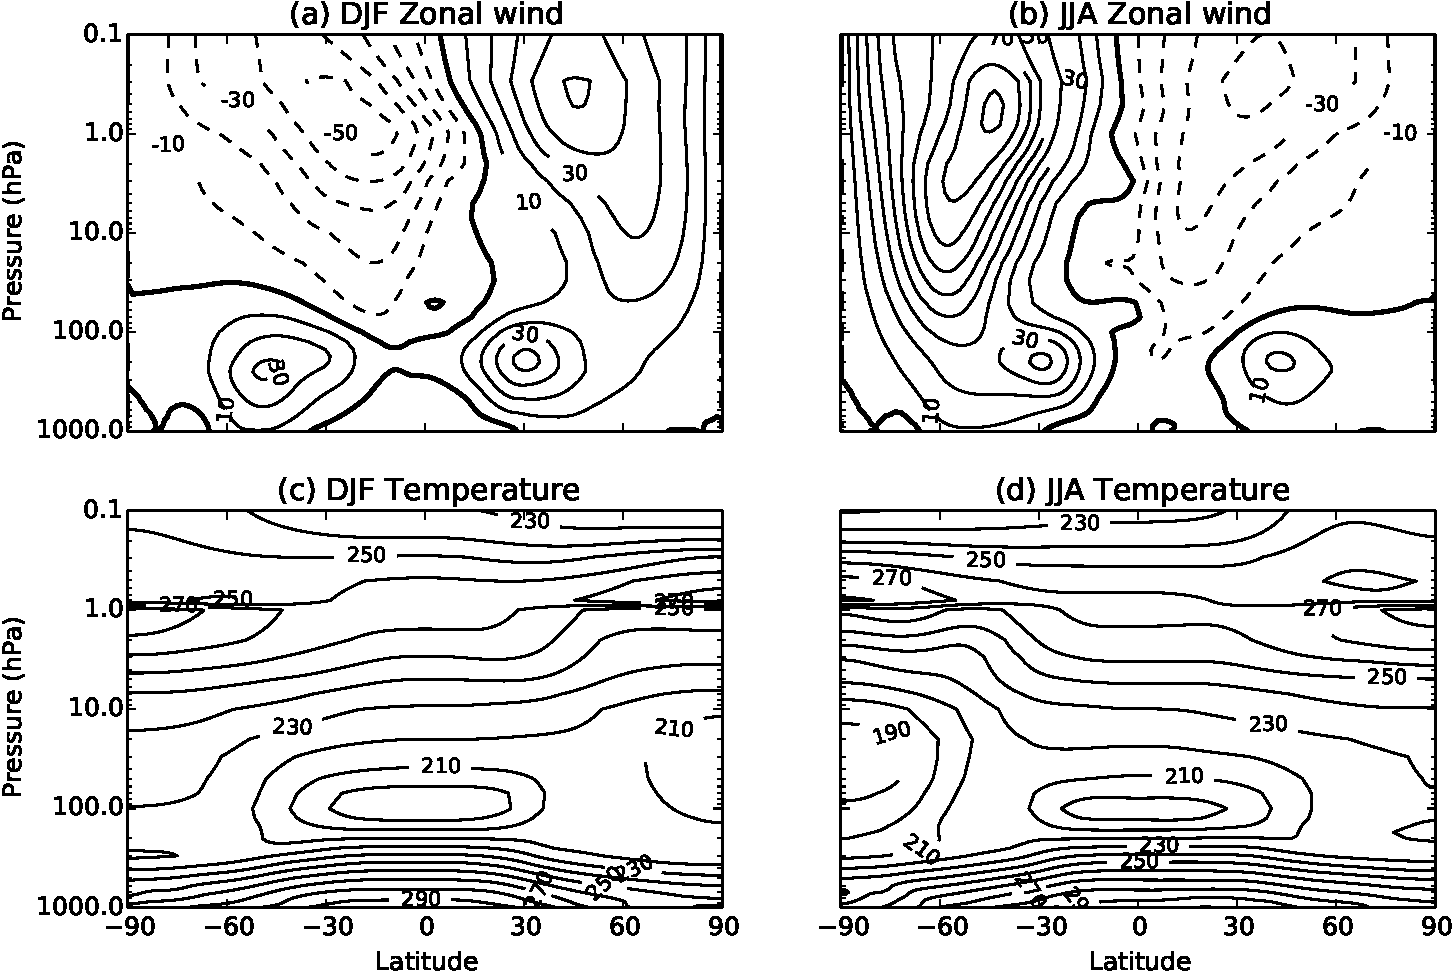
\includegraphics[width=\textwidth]{figures/chapter-intro/zmzw_zmT_clim.pdf}
 \caption[Zonal-mean zonal wind and temperature climatology]{December-January
   (DJF) (a,c) and July-August (JJA) (b,d) averages of zonal-mean zonal wind
   ($\mathrm{m~s^{-1}}$) (a,b) and temperature (K) (c,d). Dashed contours
   represent negative values. Data is from the ERA-Interim reanalysis
   (1979--2010).}
 \label{fig:zmzw_zmT_clim}
\end{figure}

Figure \ref{fig:zmzw_zmT_clim} shows zonal-mean zonal wind and temperature
averaged over the boreal winter (December--February; DJF) and austral winter
(July--August; JJA) using data from 1979--2010 from the ERA-Interim reanalysis
(details in Section \ref{sec:reanalysis-data}). In both cases the westerly
vortex in the winter hemisphere can be seen along with a local minimum in
temperature at the winter pole in the lower stratosphere. Easterly winds are
present in the summer hemisphere. The maximum strength of the polar vortex
occurs at midlatitudes between 0.1--1~hPa in the mesosphere, and is stronger in
the Southern Hemisphere (SH) with a maximum of $90~\mathrm{ms^{-1}}$ than the
Northern Hemisphere (NH) with a maximum of $50~\mathrm{ms^{-1}}$. The winter
polar stratosphere is also approximately $20$~K colder in the SH than the NH.

\begin{figure}
 \centering
 \noindent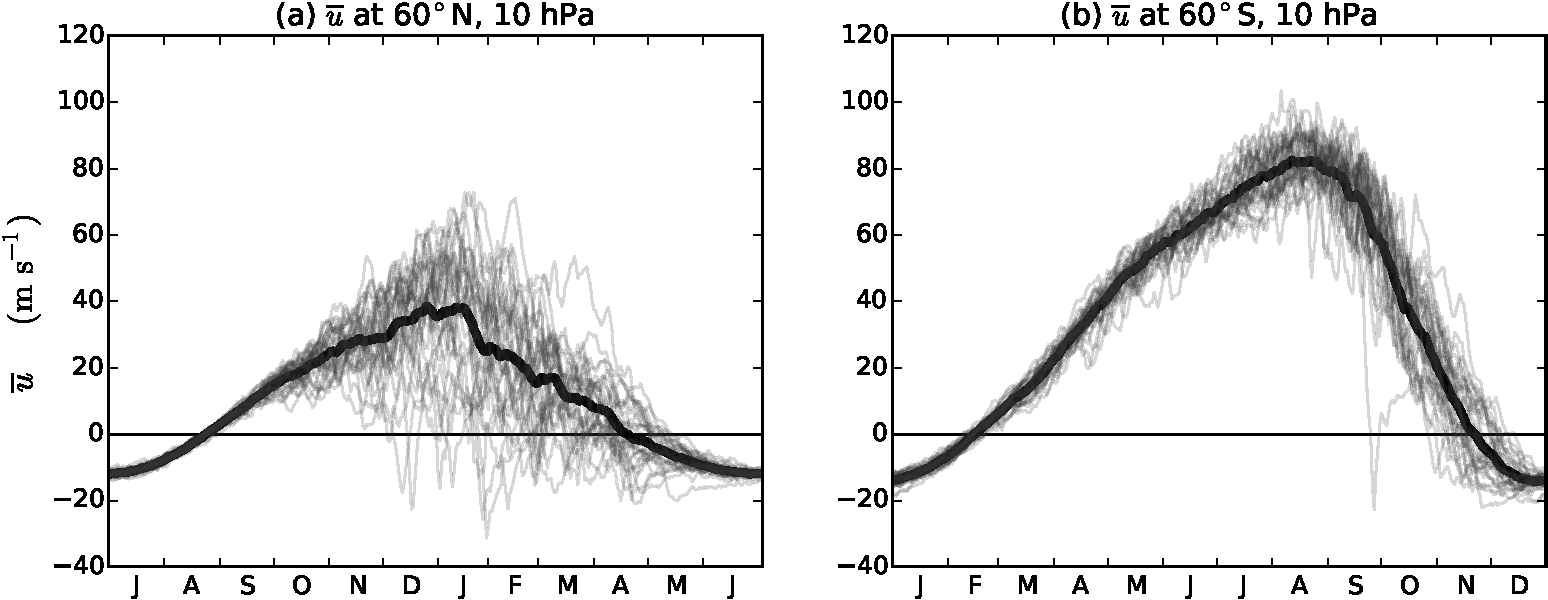
\includegraphics[width=\textwidth]{figures/chapter-intro/zmzw_NH_SH_fix.pdf}
 \caption[Comparison of NH and SH polar vortex seasonal cycle]{Seasonal cycle
   of NH (a) and SH (b) polar vortex strength, measured by $\overline{u}$ at
   60$^{\circ}$N/S, 10~hPa. The annual mean is shown in a thick black line and
   individual years in thin grey lines. Both time series are centred on their
   respective winters. Data is from the ERA-Interim reanalysis (1979--2010).}
 \label{fig:zmzw_NH_SH}
\end{figure}

The maximum strength of the vortex in the stratosphere occurs at approximately
$60^{\circ}$N/S with little variation through the depth of the
stratosphere. Figure \ref{fig:zmzw_NH_SH} shows the annual cycle and variability
of zonal-mean zonal wind at $10$~hPa $60^{\circ}$N and $60^{\circ}$S. As well as
being weaker on average than the SH, the winter NH stratospheric polar vortex
can also be seen to be significantly more variable than the SH. There are a
number of years in the NH for which $\overline{u}$ becomes negative during the
winter, but only one such year in the SH (these events are discussed further in
Section \ref{sec:strat-sudd-warm}). A further clear feature of both NH and SH is
that variability during the summer is much less than that during winter. Also,
the transition to summer easterlies (known as the final warming) occurs
relatively earlier in the seasonal cycle in the NH than the SH. All these
observations are due almost entirely to the influence of wave phenomena in the
stratosphere, as described in the next section.


\subsection{Waves in the stratosphere}
\label{sec:plan-waves-strat}

\subsubsection{Planetary waves}
\label{sec:planetary-waves}

Large-scale Rossby or planetary waves\footnote{Here, as is common in the
  stratospheric literature, ``wave'' is taken to mean any deviation from the
  zonal-mean state.} play a vital
role in the dynamics of the extratropical stratosphere. They mostly enter the
stratosphere from the troposphere, where they are forced, for example, by air
flow around topography, latent heat release, or nonlinear evolution of
tropospheric eddies \citep{Scinocca1998}. These large-scale waves approximately
satisfy the quasi-geostrophic (QG) approximation of hydrostatically balanced
incompressible flow with low Rossby number, $\mathrm{Ro} = U/f_oL \ll 1$, where
$U$ and $L$ are characteristic velocity and length scales respectively
\citep{Andrews1987}. Under this approximation and in the absence of friction,
the following relation, known as the \emph{quasi-geostrophic potential vorticity
  equation}, holds:
\begin{equation}
D_gq_g = f_0\rho_0 \frac{\partial}{\partial z}
\frac{\rho_0Q}{\partial\theta_{0}/\partial z} \, . 
\label{eq:qgpv}
\end{equation}
Where
\begin{equation}
D_g \equiv \frac{\partial}{\partial t} + u_g\frac{\partial}{\partial x} +
v_g\frac{\partial}{\partial y} \, , 
\end{equation}
and 
\begin{equation}
  q_g = f_0 + \beta y - \frac{\partial v_g}{\partial x} + \frac{\partial u_g}{\partial
    y} + \rho_o^{-1}\frac{\partial}{\partial
    z}\left(\rho_of_0\frac{\theta_e}{\partial\theta_{0}/\partial z}\right) \, , 
\end{equation}
is the quasi-geostrophic potential vorticity. Here, $v_g$ is the geostrophic
meridional velocity, $v_g = f^{-1}\partial Z/\partial x$, $Q$ is the diabatic
heating rate, $\rho_0$ is a reference density and $\theta_0$ is a reference
potential temperature, $\theta_0 = T_s(p_s/p)^\kappa$, where
$p_s=1000~\mathrm{hPa}$, and $\kappa = R/c_p \approx 2/7$, where $c_p$ is the
specific heat capacity of air at constant pressure. $\theta_e$ represents the
departure from $\theta_0$, and is assumed to be small in the sense that
$|\partial\theta_e/\partial z| \ll |\partial\theta_0/\partial z|$. An important
consequence of Equation \ref{eq:qgpv} is that $q_g$ is conserved following the
geostrophic wind for adiabatic flow ($Q=0$), and therefore acts as a
tracer\footnote{Throughout most of this thesis, Ertel's potential vorticity,
  $q$, is used. This is defined by
\begin{equation*}
  q = \frac{1}{\rho}\zeta\cdot\nabla\theta \, , 
\end{equation*}
where
$\zeta$ is the absolute vorticity. \citet{Charney1962} showed that when the
quasi-geostrophic approximation is valid
\begin{equation*}
\left(\frac{\partial q}{\partial s}\right)_{\theta=\mathrm{const.}} \approx
\frac{1}{\rho_0}\frac{\partial \theta_0}{\partial z}\left(\frac{\partial
    q_g}{\partial s}\right)_{z=\mathrm{const.}} \, ,
\end{equation*}
where $s = t$, $x$ or $y$. Hence, a similar conservation law as for
$q_g$ applies to $q$, which is conserved on isentropic (e.g., constant
$\theta$) surfaces.  }.

In the case of approximately zonal flow $[\overline{u}(y,z),0,0]$, Equation
\ref{eq:qgpv} can be linearised to give
\begin{equation}
\left(\frac{\partial}{\partial t} + \overline{u}\frac{\partial}{\partial
    x}\right)q_g' + v'\frac{\partial\overline{q_g}}{\partial y} = f_0\rho_0 \frac{\partial}{\partial z}
\frac{\rho_0Q'}{\partial\theta_{0}/\partial z} \, ,
\label{eq:linear_qgpv} 
\end{equation}
where primes represent deviations from the zonal mean (e.g., $q_g =
\overline{q_g} + q_g'$). It can be shown that Equation \ref{eq:linear_qgpv}
supports wave-like solutions, with vertical propagation dependent upon the
condition:
\begin{equation}
0 < \overline{u}-c < \overline{u}_c \equiv \beta(k^2+l^2+\varepsilon/4H^2)^{-1} \,,
\end{equation}
which is known as the \emph{Charney-Drazin criterion} after
\citet{Charney1961}. Here, $c$ is the wave's zonal phase speed, $k$ and $l$ are
the zonal and meridional wavenumbers respectively, and
$\varepsilon = f_0^2/N^2$, where
$N^2 = H^{-1}Re^{-\kappa z/H}\partial\theta_0/\partial z$ is the static
stability. $H$ is the pressure scale height, $H=RT_s/g$, where $g$ is the
acceleration due to gravity and $T_s$ is a reference temperature. In the case of
waves whose phase is stationary with respect to the ground ($c=0$), this
simplifies to
\begin{equation}
0 < \overline{u} < \overline{u}_c\, . 
\label{eq:charney-drazin}
\end{equation}
It is therefore apparent that in order for planetary waves to propagate
vertically (such as from the troposphere to the stratosphere), a westerly flow
must be present that is not too strong. Additionally, this maximum speed is
dependent on wavenumber, such that a lower wavenumber can propagate in a
stronger westerly flow. While the assumptions here are not representative of the
real atmosphere (such as purely zonal flow, and small deviations from the zonal
mean), this criterion does capture the most important features of the relation
between zonal assymmetries and the zonal flow, and similar relations can be
found for more complex background states \citep{Andrews1987}.

An important consequence of the Charney-Drazin criterion for stratospheric flow
is that the strength of the stratospheric polar vortices shown in Figures
\ref{fig:zmzw_zmT_clim} and \ref{fig:zmzw_NH_SH} is often sufficient to exclude
all but the lowest wavenumbers (typically zonal wavenumbers 1--3; hereafter
referred to as `wave-$n$') from propagating upwards from the troposphere. Hence
the length-scale of typical stratospheric zonal asymmetries is much larger than
that of the troposphere.

\bigskip When planetary waves reach a \emph{critical surface}, where propagation
is prohibited (for instance, a region where $\overline{u} = c$), the above
linear analysis breaks down. In this scenario waves can ``break'', imparting
momentum onto the zonal flow. There is therefore a two-way interaction between
the zonal flow and planetary waves; a phenomenon known as \emph{wave-mean flow
  interaction}. Wave breaking was studied in an idealised two-dimensional model
by \citet{Stewartson1978} and \citet{Warn1978}. They found momentum to be
absorbed in a narrow \emph{critical layer} close to the critical surface, with
potential vorticity (PV) contours being irreversibly stretched and mixed in
increasingly fine scales; a process known as a `potential enstrophy cascade'
\citep[e.g.,][]{Rhines1979}. They also showed that the critical layer is
initially absorbing, but becomes a reflecting surface after some time. Time
varying results from a version of the Stewartson-Warn-Warn model from
\citet{Andrews1987} are shown in Figure \ref{fig:cats_eyes}. Similar wave
breaking behaviour was first observed in the real stratosphere by
\citet{McIntyre1983} using isentropic maps of Ertel's potential vorticity,
including the irreversible deformation of PV contours of the kind shown in
Figure \ref{fig:cats_eyes}.

\begin{figure}
 \centering
 \noindent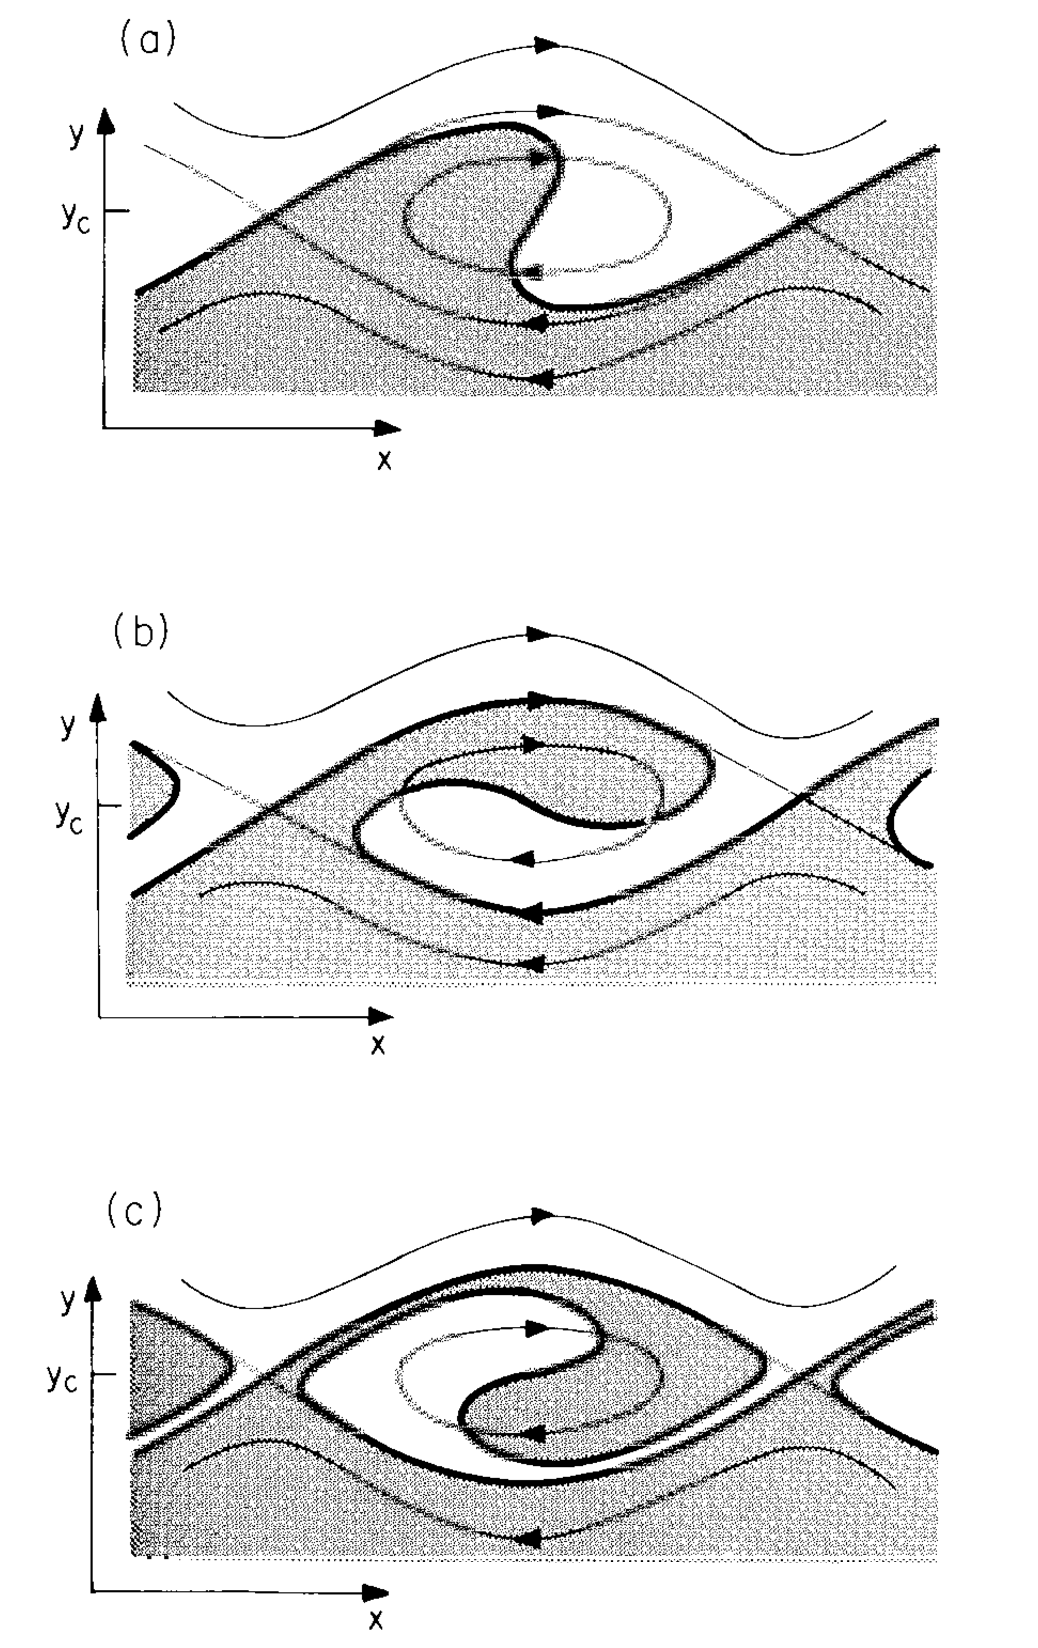
\includegraphics[width=0.6\textwidth]{figures/chapter-intro/breaking_wave_AHL.pdf}
 \caption[Results from a Stewartson-Warn-Warn model of wave
 breaking]{Stewartson-Warn-Warn time-dependent analytical solution of a Rossby
   wave nonlinear critical layer (time advancing in even steps from
   (a)-(b)-(c)). The flow is periodic in $x$ and the $y$ scale is greatly
   exaggerated and the initial critical line was at $y=y_c$. The thin lines
   indicate streamlines and lens shaped regions of closed streamlines are known
   as ``Kelvin's cats' eyes''. The thick line shows the position of the absolute
   vorticity contour $\zeta=\zeta_c$, that initially lay along $y=y_c$ (in this
   barotropic model, the quasi-geostrophic potential vorticity, $q_g$, reduces
   to $\zeta$). Hence, $\zeta<\zeta_c$ in the stippled region and
   $\zeta>\zeta_c$ in the unstippled region. In (a) it can be seen that $v>0$
   for most of the stippled region, indicating partial absorption, whereas in
   (b) and (c) $v\leq0$ in the stippled region indicating reflection. Figure
   from \citet{Andrews1987}.}
 \label{fig:cats_eyes}
\end{figure}

A further effect of wave breaking is the induction of a \emph{residual
  circulation}, $[0, \overline{v}^*, \overline{w}^*]$, where $\overline{v}^*$ and
$\overline{w}^*$ are the transformed Eulerian-mean (TEM) meridional and vertical
velocities given in spherical coordinates by
\begin{equation}
  \overline{v}^* = \overline{v} - \frac{1}{\rho_0}\frac{\partial}{\partial z}
  \left(\frac{\rho_o\overline{v'\theta'}}{\partial\overline{\theta}/{\partial z}}\right) \, , 
\end{equation}
\begin{equation}
\overline{w}^* = \overline{w} + \frac{1}{a\cos\phi}\frac{\partial}{\partial\phi}
\left(\frac{\cos\phi\overline{v'\theta'}}{\partial\overline{\theta}/{\partial
      z}}\right) \, ,
\end{equation}
which approximates the Lagrangian-mean circulation under time-averaged
conditions \citep{Andrews1976,Dunkerton1978,Holton1990}. Under the TEM
formalism, the zonal momentum equation becomes
\begin{equation}
\frac{\partial\overline{u}}{\partial t} +
\overline{v}^*\left(\frac{1}{a\cos\phi}\frac{\partial}{\partial\phi}(\overline{u}\cos{\phi})
  - f \right) + \overline{w}^*\frac{\partial\overline{u}}{\partial z} =
\frac{\mathbf{\nabla \cdot F}}{\rho_oa\cos\phi} + \overline{X} \equiv \overline{\mathcal{F}}
\label{eq:zonal_momentum}
\end{equation}
where $\overline{X}$ represents frictional terms and $\mathbf{F}=[0,F^\phi,F^z]$
is the Eliassen-Palm (EP) flux with components
\begin{equation}
F^\phi = \rho_0a\cos\phi\left(\frac{\partial\overline{u}}{\partial
    z}\frac{\overline{v'\theta'}}{\partial\overline{\theta}/\partial z} -
  \overline{v'u'}\right) \, ,
\end{equation}
\begin{equation}
F^z =
\rho_0a\cos\phi\left(\left[f-\frac{1}{a\cos\phi}\frac{\partial}{\partial\phi}(\overline{u}\cos\phi)\right]\frac{\overline{v'\theta'}}{\partial\overline{\theta}/\partial
      z} - \overline{w'u'}\right) \, .
\end{equation}
$\mathbf{F}$ can be interpreted as the flux of wave activity
\citep{Andrews1987}, and therefore $\mathbf{\nabla\cdot F}<0$ (convergence)
represents a dissipation of wave activity, as is the case in wave breaking. It
can be seen that for a steady zonal flow ($\partial\overline{u}/\partial t = 0$)
in the absence of wave driving ($\mathbf{\nabla\cdot F} = 0$) or friction
($\overline{X} = 0$), a solution of Equation \ref{eq:zonal_momentum} is
$\overline{v}^*=0, \overline{w}^*=0$.  However, in the presence of these forcing
terms, a non-zero residual circulation will be induced. Climatologically, this
circulation consists of wave-driven poleward and downward motion in the
extratropics which is balanced by upwelling in the tropics. This diabatic
circulation (i.e., the transport of mass accross isentropic surfaces) forms a
significant part of the Brewer-Dobson circulation\footnote{Strictly, the
  Brewer-Dobson circulation represents the meridional transport of tracers, and
  so also involves two-way isentropic mixing (i.e. transport without net
  transfer of mass), which is an adiabatic process \citep{Hall1994}.}. The
downward motion near the poles can be easily seen from Equation
\ref{eq:zonal_momentum} in the steady case; since $\overline{v}^*$ must become
small near the poles (by conservation of mass), and
$\partial\overline{u}/\partial z > 0$ in the polar vortex, if
$\mathbf{\nabla\cdot F} < 0$, then $\overline{w}^*<0$. It is observed that this
circulation is strongest in the winter hemisphere due to the fact that more
planetary waves can propagate and break in the winter westerly flow than the
summer easterly flow (due to the Charney-Drazin criterion). Furthermore, during
periods of enhanced wave breaking the residual circulation accelerates and there
is more descent and adiabatic heating at high latitudes. This is important in
the physical understanding of sudden stratospheric warming events, described in
Section \ref{sec:strat-sudd-warm}.


\subsubsection{Gravity waves}

Gravity waves are another type of atmospheric wave important in the dynamics of
the polar stratosphere. These waves owe their existence to buoyancy restoring
forces and can be generated by a number of processes such as air flow over
topography (orographic gravity waves), convection or frontogenesis
(non-orographic gravity waves). As with planetary waves, the differences in the
land masses of the two hemispheres leads to orographic gravity wave activity
being much greater in the NH. These waves make a net easterly contribution to
the winter zonal flow \citep[e.g.,][]{Seviour2012}, and so act to enhance the
residual circulation. Their typical length scales are much shorter than can be
resolved in general circulation models or reanalyses, and so they are usually
parametrised, appearing as the term $\overline{X}$ in the zonal momentum
equation (Equation \ref{eq:zonal_momentum}).
\begin{center}
\line(1,0){250}
\end{center}

\bigskip Together, the Charney-Drazin criterion and the effects of planetary and
gravity wave driving on the zonal flow can expain almost all hemispheric
differences seen in Figures \ref{fig:zmzw_zmT_clim} and \ref{fig:zmzw_NH_SH}:
Greater topography results in more planetary and gravity wave generation in the
NH, both of which cause a net deceleration of the westerly polar vortex, thereby
causing the NH vortex to be weaker than the SH. This also explains why the NH
vortex is warmer than the SH, as the greater NH wave activity induces a stronger
residual circulation with enhanced descent and adiabatic warming at high
latitudes. Additionally, the strength of the SH vortex is such that it prohibits
the vertical propagation of planetary waves from the troposphere throughout much
of the winter, meaning that the SH vortex is less variable than the NH. Both
hemispheres show very little variability in the summer easterly flow because
planetary wave propagation is prohibited in this regime.


\subsection{Sudden stratospheric warmings}
\label{sec:strat-sudd-warm}
%footnote on name
First observed by \citet{Scherhag1952} in radiosonde measurements over Berlin,
the extreme events visible in Figure \ref{fig:zmzw_NH_SH} whereby the winter
circulation temporarily becomes easterly\footnote{For a discussion of more
  precise definitions of SSWs, see Section \ref{sec:moments-introduction}.} are
known as sudden stratospheric warmings\footnote{Following \citet{Butler2014a} it
  is suggested that the term \emph{sudden stratospheric warming} is preferable
  to the common alternative \emph{stratospheric sudden warming}. This is because
  there are other varieties of stratospheric warming (such as final warmings or
  Canadian warmings), but not other varieties of atmospheric sudden warming.}
(SSWs). These events occur approximately 5--7 times per decade in the NH, but
only one such event has been observed in the almost 60 year observational record
in the SH (in 2002). They are called ``warmings'' because associated with the
circulation reversal is a dramatic increase in temperature; as much as 50~K in
the space of a few days in the mid-stratosphere.\footnote{A recent study
  \citep{Neef2014} has even suggested that SSWs have a sufficiently strong
  influence on the Earth's angular momentum that they have a detectable
  influence on the length of the day.}

Initially these events were thought to result from either solar storms
\citep{Scherhag1952} or baroclinic instability of the stratospheric polar vortex
\citep{Murray1960}. However, \citet{Matsuno1970, Matsuno1971} proposed a model
of SSWs which relies on the influence of tropospherically forced planetary
waves. This model (or modifications thereof) remains the most widely accepted
dynamical view of SSWs at present. The mechanism proceeds as follows:
\begin{enumerate}[i.]
\item A packet of enhanced planetary wave activity enters the stratosphere where
  it reaches a critical surface and breaks. This decelerates the zonal flow over
  a broader critical layer, and if strong enough causes it to reverse.
\item Hence a new critical surface is formed at a lower level (where
  $\overline{u}=0$), and wave breaking occurs at this level. The process
  continues as the critical layer descends to the lower stratosphere.
\item At the same time, wave breaking induces an enhanced residual circulation
  with greater descent and adiabatic warming at high latitudes. If strong
  enough, this can act to reverse the meridional temperature gradient, further
  enhancing the easterly flow by thermal wind balance. 
\item When the critical surface is close to the tropopause, planetary wave
  activity is essentially prohibited from entering the polar
  stratosphere. Radiative cooling to space then acts to cool the polar
  stratosphere and the vortex reforms over a period of approximately 2--4 weeks.
\end{enumerate}

This mechanism considers the effect of planetary waves on the zonal-mean
flow. However, it has been observed that SSWs generally occur as either a split
or displacement of the vortex, mostly depending (though not exclusively; see
Section \ref{sec:moments-introduction}, \citep{Waugh1997}) on whether wave-2 or
wave-1 activity is dominant. An example of each of these events is shown in
Figure \ref{fig:charlton_polvani_ssw}. \citet{Charlton2007} and
\citet{Matthewman2009} studied the dynamics of these two types of events in
reanalysis data and noted some differences. Most significantly, split vortex
events were observed to occur near-barotropically, with two smaller vortices
centred over Canada and Siberia throughout the depth of the stratosphere. On the
other hand, displaced vortex events were observed to be more baroclinic,
starting first in the upper stratosphere with a vortex centred over Canada, the
centre of which rotates westward with height and is centred over Siberia in the
lower stratosphere.


\begin{figure}
 \centering
 \noindent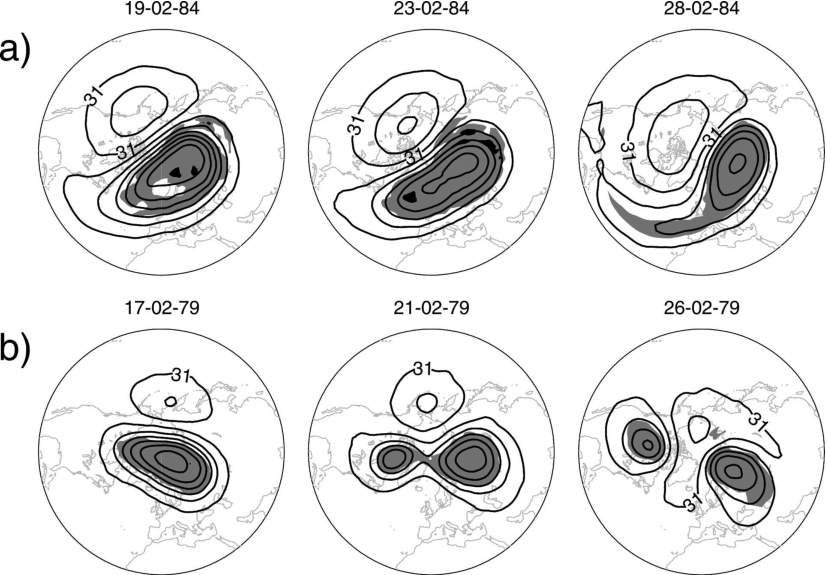
\includegraphics[width=\textwidth]{figures/chapter-intro/charlton_polvani_SSW.pdf}
 \caption[A split and displaced vortex event from \citet{Charlton2007}]{Polar
   stereographic plot of geopotential height (contours) on the 10~hPa pressure
   surface. The contour interval is 0.4~km, and shading shows potential
   vorticity greater than $4.0 \times 10^{-6}
   \mathrm{K~kg^{-1}~m^2~s^{-1}}$.
   (a) A vortex displacement type warming that occurred in February 1984. (b) A
   vortex splitting type warming that occurred in February 1979. Figure from
   \citet{Charlton2007}.}
 \label{fig:charlton_polvani_ssw}
\end{figure}

This different behaviour of split and displaced vortex events is not accounted
for by the \citet{Matsuno1970, Matsuno1971} model above, and so may suggest that
other mechanisms are important in the generation of SSWs. For instance,
\citet{ONeill1988} and \citet{Scott2006} have suggested that SSWs can be
generated by a cyclone-anticyclone interaction between the Aleutian high and the
polar vortex. These studies showed that a smaller anticyclone can act to
significantly distort the polar vortex, although such interactions are greatest
for circulation ratios higher than are typically found in the polar
stratosphere. Other studies have suggested that SSWs can arise through the
resonant excitation of normal modes of the stratosphere by planetary waves
\citep{Tung1979}. Significantly, \citet{Plumb1981} found that the planetary wave
forcing need not be at exactly the resonant frequency of the mode (an occurrence
which is probably unlikely), but that the two can be brought to resonance by a
process known as nonlinear self-tuning. \citet{Smith1989} found behaviour
suggestive of this process in simulations of a SSW. More recently
\citet{Esler2005}, \citet{Esler2006}, and \citet{Matthewman2011} have argued
that a relevant mode in the case of split vortex events is the barotropic mode
of the atmosphere, which may explain the more barotropic nature of split vortex
events.\footnote{In an idealised modelling study, \citet{Esler2011} also
  suggested that resonant excitation of the first baroclinic mode may play an
  important role in the occurrence of displaced vortex events.}
\citet{Albers2014} further suggested that gravity waves play an important role
in `tuning' the geometry of the vortex towards a state in which resonance can
occur.

Further weight is given to these mechanisms which do not rely on strong
transient tropospheric forcing by the occurrence of the 2002 SH SSW, since this
forcing is much weaker in the SH (several studies of the dynamics of this event
can be found in the March 2005 special issue of \emph{Journal of Atmospheric
  Sciences}). Indeed, \citet{Esler2006} provided evidence that this event may
have been influenced by resonant excitation of the barotropic mode.

%It should also be noted that other studies have suggested that SSWs can occur
%even in the case of no tropospheric stationary forcing \citep{Kushner2005}.

Several studies have also discussed the role of the polar vortex being in a
favourable (or `preconditioned') state prior to SSWs
\citep[e.g.,][]{McIntyre1982}. In a simple dynamical model, \citet{Scott2004}
demonstrated that planetary wave breaking is enhanced by the presence of steep
PV gradients at the vortex edge, which are likely to be present in an
anomalously strong vortex. Indeed, \citet{Limpasuvan2004} found evidence for an
anomalously strong vortex 30-40 days prior to SSWs, while \citet{Charlton2007}
found this effect to be stronger prior to split vortex events than displaced
vortex events. 

Overall, while significant advances in understanding the dynamics of SSWs have
been made, several uncertainties remain. Tropospherically-driven wave activity
is certainly an important factor but the roles (if any) of cyclone-anticyclone
interactions or resonance are less certain. Moreover, it is not clear whether
different mechanisms may be more or less important in driving split and
displaced vortex events.


\section{Polar stratospheric ozone depletion}
\label{sec:polar-strat-ozone}

The Antarctic ozone hole is a large region of severely depleted ozone
concentrations in the lower-mid stratosphere which occurs during the austral
spring. During its formation ozone is often be completely destroyed at some
altitudes. A similar, but much smaller depletion is observed in the NH
\citep[e.g.,][]{Manney1997}. Following its discovery by \citet{Farman1985}, a
chemical and dynamical theory of the ozone hole was rapidly developed which
largely attributes this rapid ozone depletion to the presence of anthropogenic
chlorofluorocarbon (CFC) compounds \citep{McElroy1986,Solomon1986}. This theory
is summarised as follows:
\begin{enumerate}[i.]
\item The strong zonal winds of the stratospheric polar vortex act to confine
  air over the polar regions, with little mixing with midlatitudes
  \citep{Schoeberl1991}. This results in a region of very cold temperatures
  which allow the formation of polar stratospheric clouds (PSCs; these require
  temperatures below approximately 195~K to form \citep{Newman2010}).
\item Heterogeneous chemical reactions can take place on the surface of PSCs which
  act to convert `reservoir' chlorine species such as \ce{ClONO2} and \ce{HCl}
  into forms that can accelerate ozone depletion, for instance
  \citep{Solomon1986}:
  \begin{equation*}
    \ce{ClONO2 + HCl ->[\ce{PSC}] Cl2 + HNO3}
  \end{equation*}
\item As sunlight returns to the vortex region in spring, \ce{Cl2} is rapidly
  photolysed and reacts with oxygen to form \ce{ClO}. This can then
  catalytically destroy ozone through a reaction sequence such as the following
  suggested by \citet{Molina1987}:
  \begin{align*}
    \cee{ClO + ClO &->[\ce{M}] ClOOCl \\
         ClOOCl + $h\nu$ &-> ClOO + Cl \\
         ClOO &->[\ce{M}] Cl + O2 \\
         2(Cl + O3 &-> ClO + O2) \\
         $\mathrm{Net:~}$ 2O3 &-> 3O2} 
  \end{align*}
  where $\nu$ is the frequency of light,
  $h$ is Planck's constant, and M a third body (necessary for conservation of
  momentum). Several other reaction sequences are also possible, for instance
  involving bromine species.

\item A further effect of PSCs is that their particles fall out of the
  stratosphere and thereby remove nitrogen compounds
  (\ce{NO$_x$}) from the polar lower stratosphere \citep{Toon1986}.
  \ce{NO$_x$} compounds are important because they can react with with \ce{ClO}
  to form reservior compounds. For instance the reaction
  \begin{equation*}
    \ce{ClO + NO2 ->[\ce{M}] ClONO2}
  \end{equation*}
  removes \ce{ClO} from the ozone-depleting sequence above. Hence a reduction of
  \ce{NO$_x$} due to PSCs leads to an increase in ozone depletion.

\item After some time, radiative heating of the stratosphere is sufficient to
  prevent the formation on PSCs, so ozone depletion halts. This heating is
  further accelerated by the increased wave breaking in the polar stratosphere
  which can take place as the vortex weakens (due to the Charney-Drazin
  criterion) and thereby induce an enhanced residual circulation. Following the
  final breakdown of the vortex and transition to summer easterlies (final
  warming), the ozone-depleted air is mixed to lower latitudes.
\end{enumerate}

\begin{figure}
 \centering
 \noindent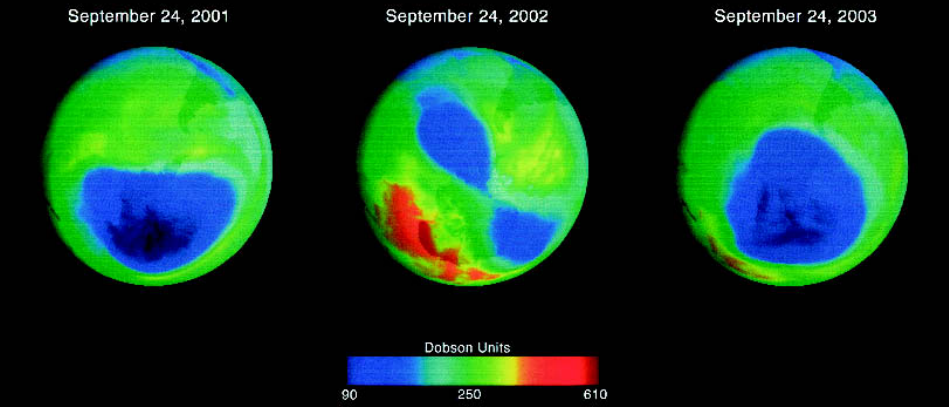
\includegraphics[width=\textwidth]{figures/chapter-intro/2002_SSW.png}
 \caption[]{Comparison of the (middle) first split ozone hole on record (2002)
   and (left) the Antarctic ozone hole at the same time one year earlier (2001)
   and (right) one year later (2003). The hole is dark blue and magenta. In
   2001, the ozone layer thinning over Antarctica reached
   $26.5 \times 10^6~\mathrm{km^2}$ , larger than the size of the entire North
   American continent. Due to higher Antarctic winter temperatures, the 2002
   ``hole'' seems to be about 40\% smaller. In 2003, Antarctic winter
   temperatures returned to normal and the ozone hole returned to its usual
   state. Figure from \citet{Shepherd2005}.}
 \label{fig:2002_SSW}
\end{figure}

Importantly, the stratospheric dynamics described in Section
\ref{sec:dynam-polar-strat}, play an important role in ozone depletion. As
discussed in Section \ref{sec:planetary-waves}, wave breaking in the
stratosphere acts to drive a residual circulation, with descent and adiabatic
warming over the pole. Enhanced descent and warming over the pole acts to
inhibit the formation of PSCs which are necessary for the above heterogeneous
chemical reactions which cause ozone depletion. A stronger meridional
circulation also acts to transport more tropical ozone-rich air to the polar
regions, further acting to increase ozone concentrations. Another mechanism in
which wave breaking acts to inhibit ozone depletion is by actively stripping
away filaments of ozone-depleted air from the polar vortex \citep{Waugh1994}. It
is this greater wave activity in the NH then that explains why the extent of
ozone depletion is much less in the NH than the SH.

%Moreover, it has been demonstrated that interannual variability in wave driving
%can account for most of the interannual variability of ozone depletion through
%this mechanism \citep{Salby2012}.

In the extreme event of SSWs, the ozone hole can be severely disrupted. This can
be seen in Figure \ref{fig:2002_SSW}, where a clear split of the ozone hole is
visible during the 2002 SH SSW, which contrasts with the more zonally symmetric
distributions seen at the same times in 2001 and 2003. The magnitude of the 2002
ozone hole can also be seen to be reduced; a result of an enhanced residual
circulation causing warmer stratospheric temperatures. The importance of this
link between dynamics and chemistry for predicting interannual variability in
ozone depletion is discussed further in Sections \ref{sec:ozone-depletion} and
\ref{sec:seas-discussion}.

\section{Annular modes}
\label{sec:annular-modes}
Before discussing the influence of the stratosphere on the troposphere, it is
necessary to introduce the concept of the annular modes which are often analysed
in studies on this topic (as well as in this thesis). The northern and southern
annular modes (NAM and SAM) are the leading modes of large-scale variability in
the two hemispheres
\citep{Thompson1998,Baldwin1999,Thompson2000a,Thompson2000,Limpasuvan1999,Limpasuvan2000}. They
are commonly defined to be the leading empirical orthogonal function
(EOF)\footnote{EOFs are the eigenvectors of the spatially weighted covariance
  matrix of a variable. EOF analysis is also known as principal component
  analysis \citep{Wilks}.} of extratropical monthly-mean geopotential height
calculated at each pressure surface \citep[e.g.,][]{Baldwin1999}, with an index
of the respective principal component or the projection of daily data onto the
EOF pattern. \citet{Baldwin2009} introduced an alternative using zonal-mean
geopotential height, which is therefore less computationally expensive to
calculate. The annular modes at the surface are also often calculated from mean
sea-level pressure \citep[e.g.,][]{Gong1999}, where they may also be referred to
as the Arctic and Antarctic oscillation (although in this thesis, the terms
\emph{surface NAM/SAM} are used).

Figure \ref{fig:annular_modes} shows linear regressions of zonal-mean
geostrophic winds and lower tropospheric geopotential height on the NAM and SAM
indices as defined by \citet{Thompson2000a}. It can be seen that the
near-surface NAM structure is more zonally asymmetric than the SAM, with centres
of action located over the Atlantic and Pacific oceans, and the SAM has a more
clearly `annular' structure. The vertical structure of the NAM and SAM appears
near barotropic, although with a slight poleward tilt with
height.\footnote{\citet{Thompson2014} have recently argued that the barotropic
  and baroclinic aspects of the SAM can be viewed as two independent modes of
  variability.} The magnitude of the zonal wind signature also increases with
height, reaching a maximum in the upper troposphere/lower stratosphere in the
SH, and the mid-stratosphere in the NH.

Despite this near-barotropic appearance, annular mode variability has quite
different physical interpretations in the troposphere and
stratosphere. Stratospheric variability is associated with approximately zonally
symmetric strengthening and weakening of the stratospheric polar vortex, while
tropospheric variability is more closely associated with meridional shifts in
the eddy-driven jets \citep{Limpasuvan1999}. Furthermore, stratospheric annular
mode variability is largely confined to winter, while tropospheric variability
has a much less pronounced seasonal cycle.

It can be seen from Figure \ref{fig:annular_modes}(d) that the Atlantic centre
of action of the NAM resembles the familiar North Atlantic Oscillation (NAO)
pattern. Indeed, the surface NAM and NAO have been observed to be highly
correlated \citep{Ambaum2001}. This has led to some debate as to whether the NAM
represents a physical mode of variability of which the NAO is just a regional
manifestation, or whether the NAM is simply a statistical artifact of more
regional variability \citep[e.g.,][]{Deser2000,Wallace2002}. This point is
addressed in Section \ref{sec:meas-strat-trop}.

% Mention recent thompson 2014 and baroclinic mode etc. 
\begin{figure}
 \centering
 \noindent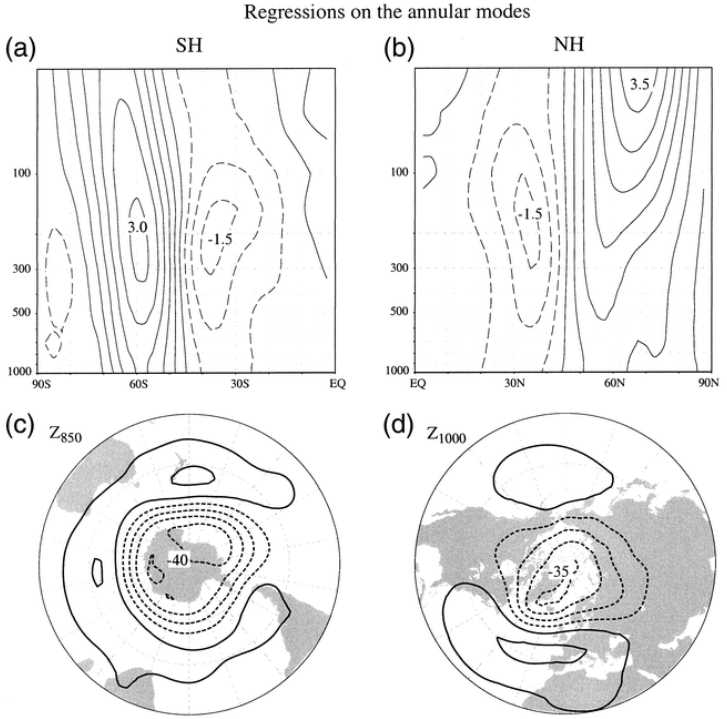
\includegraphics[width=0.7\textwidth]{figures/chapter-intro/annular_modes_TW2.png}
 \caption[Annular mode patterns from \citet{Thompson2000a}]{(top) Zonal-mean
   geostrophic wind and (bottom) lower-tropospheric geopotential height
   regressed on the standardised indices of the annular modes (the AO and its SH
   counterpart) based upon monthly data, January 1958--December 1997. Left
   panels are for the SH, right panels are for the NH. Units are
   $\mathrm{m~s^{-1}}$ (top) and m per standard deviation of the respective
   index time series (bottom). Contour intervals are 10~m ($-15,~-5,~5,~\dots$)
   for geopotential height and $\mathrm{0.5~m~s^{-1}}$ ($-0.75,~-0.25,~0.25$)
   for zonal wind. Figure from \citet{Thompson2000a}.}
 \label{fig:annular_modes}
\end{figure}


\section{Stratosphere-troposphere coupling}
\label{sec:strat-trop-coupl}

So far this chapter has dealt with the dynamics of the stratosphere as
responding passively to tropospheric forcing from below. Indeed, this was the
dominant view until the last two decades \citep[e.g.,][]{Andrews1987}. However,
observational evidence supported by modelling studies and some theoretical
arguments have now provided evidence that variability of the polar stratosphere
can significantly influence tropospheric weather and climate. This evidence is
discussed below.



\subsection{Observational evidence}
\label{sec:observ-evid}

The accumulation of observational evidence for a two-way dynamical link between
the polar stratosphere and the troposphere began in the early
1990s. \citet{Kodera1990} found that the strength of the NH upper stratospheric
polar vortex during December was correlated with the strength of the
tropospheric eddy-driven jet in February. However, they did not investigate the
mechanism for this relation, and suggested it may be radiative. Further evidence
was provided by \citet{Nigam1990} who found barotropic and baroclinic modes of
the zonal-mean zonal wind which vary coherently in the troposphere and
stratosphere. This analysis was extended by \citet{Baldwin1994} who found
significant correlations between stratospheric and tropospheric EOFs of daily NH
geopotential height (patterns which would now be referred to as annular
modes). However, they found that the strongest correlations occurred with the
troposphere leading, and while suggesting that the stratosphere may exert some
influence on the troposphere, they concluded that the direction of causality was
mostly upwards.

These studies were followed by several others which looked at the co-variability
of the stratospheric and tropospheric annular modes, and demonstrated links
between the strength of the polar vortex and surface temperature and sea level
pressure patterns \citep{Perlwitz1995, Thompson1998,Baldwin1999}. However, it
was \citet{Baldwin2001a} who first demonstrated that the
stratosphere-troposphere link is particularly strong following extreme
weakenings or strengthenings of the stratospheric polar vortex. Figure
\ref{fig:baldwin_dunkerton} shows a time series of the NAM during the winter of
1998--1999, which includes two such weak vortex events (in December and
February), characterised by a negative stratospheric NAM (these events are
highly correlated with SSWs). It is apparent that the NAM signal appears to
descend in the case of the latter event (but not the former) and consistent
anomalies remain in the troposphere for approximately one month. This timescale
is much longer than the usual timescales of tropospheric NAM variability
\citep[e.g.,][]{Simpson2011} but is more representative of the time taken for
the stratosphere polar vortex to recover following a SSW.

%\begin{figure}
% \centering
% \noindent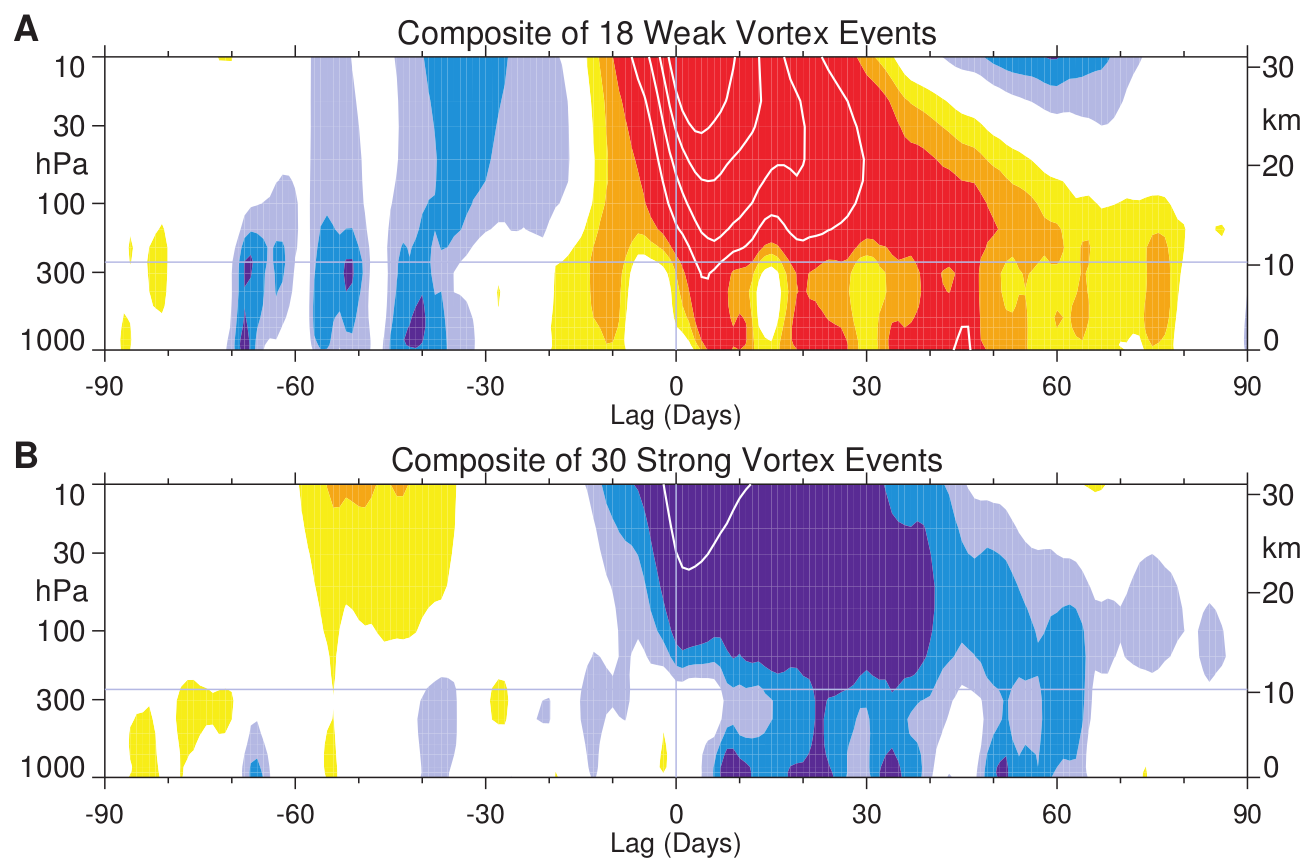
\includegraphics[width=\textwidth]{figures/chapter-intro/Baldwin_Dunkerton.png}
% \caption[NAM composite from \citet{Baldwin2001a}]{Composites of time-height
%   development of the northern annular mode for (A) 18 weak vortex events and
%   (B) 30 strong vortex events. The events are determined by the dates on which
%   the 10-hPa annular mode values cross –3.0 and +1.5, respectively. The indices
%   are nondimensional; the contour interval for the colour shading is 0.25, and
%   0.5 for the white contours. Values between −0.25 and 0.25 are unshaded. The
%   thin horizontal lines indicate the approximate boundary between the
%   troposphere and the stratosphere. Figure from \citet{Baldwin2001a}.}
% \label{fig:baldwin_dunkerton}
%\end{figure}

\begin{figure}
 \centering
 \noindent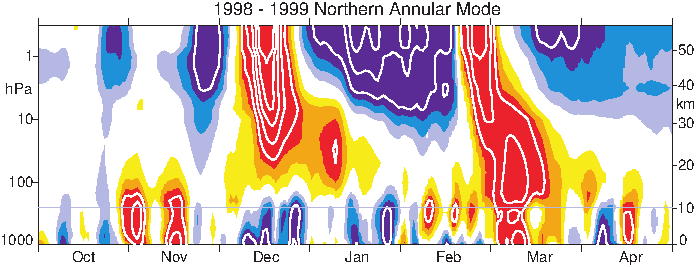
\includegraphics[width=\textwidth]{figures/chapter-intro/Baldwin_Dunkerton_98-99.pdf}
 \caption[NAM time series from \citet{Baldwin2001a}]{Time-height development of
   the northern annular mode during the winter of 1998--1999. The indices have
   daily resolution and are nondimensional. Blue corresponds to positive values
   (strong polar vortex), and red corresponds to negative values (weak polar
   vortex). The contour interval is 0.5, with values between $-0.5$ and 0.5
   unshaded. The thin horizontal line indicates the approximate location of the
   tropopause. Figure from \citet{Baldwin2001a}.}
 \label{fig:baldwin_dunkerton}
\end{figure}

Most observational studies of stratosphere-troposphere coupling have focused on
the NH because of the greater stratospheric variability there. However,
\citet{Thompson2002a} argued that a long-term strengthening of the SH
stratospheric polar vortex resulting from ozone depletion may be causing trends
in the tropospheric SAM through a dynamical link. This was supported by
\citet{Thompson2005}, who performed an analysis similar to \citet{Baldwin2001a},
finding long-lived tropospheric SAM anomalies following strengthenings and
weakenings of the SH stratospheric polar vortex (although these have a much
smaller magnitude to the NH equivalents). They also found a strong tropospheric
SAM signal following the 2002 SH SSW.

More recent studies of tropospheric anomalies following stratospheric events
have focused on more localised extreme weather events in addition to the
annular modes. Several such studies have found associations between weakenings
of the NH stratospheric polar vortex and an increased likelihood of extreme cold
events over North America, northern Europe and eastern Asia \citep{Thompson2002,
  Kolstad2010, Tomassini2012}. These extreme cold events are often linked with
persistent `blocking' weather patterns,\footnote{These are characterised by a
  persistent anticyclonic anomaly that causes a reversal in the
  upper-tropospheric meridional gradient of a quantity such geopotential height
  \citep[e.g.,][]{Tibaldi1990}.}  and a number of studies have investigated the
association between stratospheric variability and blocking. Although
\citet{Taguchi2008} found no statistically significant change in blocking
frequency during periods before or after SSWs, several studies have asserted an
upwards link, with blocking events preceding a weakened polar vortex
\citep{Quiroz1986, Andrews1987, ONeill1994}. More recent studies have further
investigated whether blocking in particular locations precedes split or
displaced vortex events, although these have reached conflicting conclusions
\citep{Martius2009, Woollings2010c, Castanheira2010}. A downwards link between
stratospheric variability and the likelihood of blocking events was suggested by
\citet{Kodera1995}. \citet{Woollings2010c} and \citet{Davini2014} have recently
found more evidence for this link, including stratosphere-leading relationships
between stratospheric variability and high-latitude blocking which may be
associated with the stratospheric impact on the tropospheric NAM. Overall
however, the nature of link between stratospheric variability and blocking
remains uncertain and is a topic of active research.

\begin{figure}
 \centering
 \noindent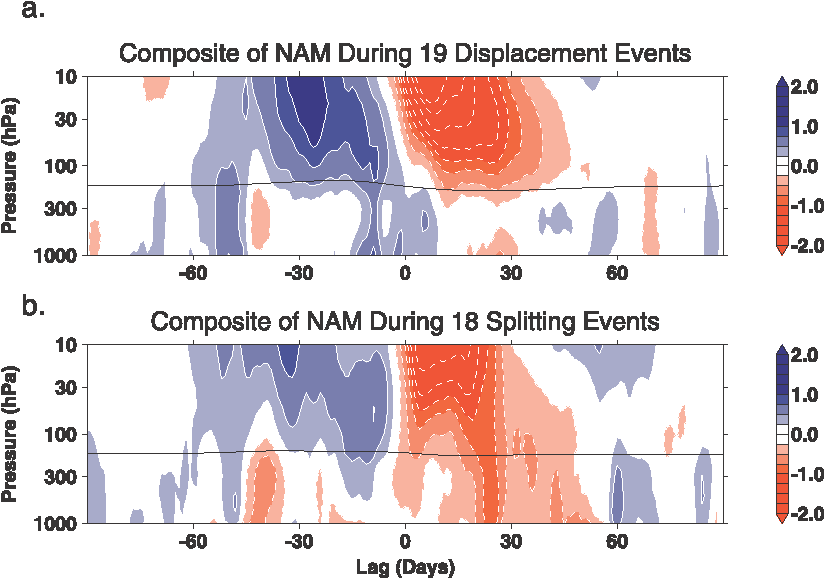
\includegraphics[width=\textwidth]{figures/chapter-intro/M13.pdf}
 \caption[NAM composite from \citet{Mitchell2013}]{Composites of the
   time--height evolution of the NAM during (a) 19 vortex displacement events
   and (b) 18 splitting events. The horizontal line is a composite of the
   thermal tropopause level for the two types of event. Lag 0 shows the onset of
   an event as measured at 10~hPa. Contour intervals are 0.25 and the region
   between $-0.25$ and 0.25 is unshaded. Figure from \citet{Mitchell2013}. }
 \label{fig:M13}
\end{figure}


It has been observed that some SSW events, while appearing to have similar
magnitudes in the stratosphere, have very different signatures in the
troposphere \citep[e.g.,][]{Baldwin2001a,Tomassini2012} (See also the two events
shown in Figure \ref{fig:baldwin_dunkerton}). This issue was addressed by
\citet{Nakagawa2006} and \citet{Mitchell2013}, who compared tropospheric
anomalies following SSWs dominated by wave-1/wave-2 activity and displaced/split
vortex events respectively (these two classifications are related but not
identical; see \citet{Waugh1997}, Section \ref{sec:comp-zonal-wave}). These
studies found stronger tropospheric anomalies following wave-2/split vortex
SSWs than following wave-1/displaced vortex SSWs.\footnote{Using the method
  developed in Chapter \ref{cha:moments}, of the two weak vortex events
  illustrated in Figure \ref{fig:baldwin_dunkerton}, the first is identified as
  a displaced vortex event and the second as a split vortex event. Their
  tropospheric NAM may therefore be expected to be different, although no firm
  conclusions should be reached from the study of just two events.} This result
is illustrated in Figure \ref{fig:M13}, which shows composites of the NAM
following the split and displaced vortex events identified by
\citet{Mitchell2013}. It can be seen that tropospheric anomalies are stronger
following split vortex events and persist for up to two months, while the NAM
signal following displaced vortex events appears not to descend below the
tropopause even though its stratospheric magnitude is
greater. \citet{Mitchell2013} went on to link these different NAM signals to an
increase in high-latitude blocking following split vortex events, and a weaker
blocking signal following displaced vortex events. On the other hand
\citet{Charlton2007}, using a different classification method, found little
difference in the tropospheric signals following split and displaced vortex
events. This discrepancy between these studies highlights the importance of the
classification method of split and displaced vortex events (or of tropospheric
variability); an issue which is addressed in Chapter~\ref{cha:moments}.

It is not only mid-winter stratospheric variability which has been suggested to
influence tropospheric weather. \citet{Hardiman2011} found differences
in NH springtime sea-level pressure anomalies following two types of
stratospheric final warming; more radiatively driven final warmings where the
transition to easterlies happens first in the upper stratosphere and descends
with time, and more dynamically driven final warmings where the transition to
easterlies happens first in the mid-stratosphere.  

A significant limitation of the above observational studies, which employ
composite or correlation analysis, is that they cannot in themselves demonstrate
\emph{causality}. For example, there may be the possibility that a third factor
(such as sea-surface temperatures) affects both the troposphere and stratosphere
separately. To address this, a number of modelling studies have been carried out
which measure the tropospheric response to some imposed stratospheric
perturbation. These are described in the next section.


% extreme events
% splits and displacements
% - + sd blocking incl Martius 2009
% hardiman fws

\subsection{Modelling evidence}
\label{sec:modelling-evidence}
Modelling investigations into a possible stratospheric influence on the
troposphere predate the observational evidence described above. In a general
circulation model (GCM) study, \citet{Boville1984} showed that changes to upper
tropospheric and lower stratospheric zonal mean zonal winds have a significant
effect on mid-troposphere wave fields, although the wind changes imposed in his
model were larger than those in reality. Using more realistic wind variations,
\citet{Jacqmin1985} found the troposphere to be largely insensitive to changes
in the state of the stratosphere. However, several more recent studies using
models with a more realistic representation of stratospheric dynamics, have
found a consistent tropospheric response to an imposed stratospheric torque
\citep[e.g.,][]{Polvani2002,Norton2003, Taguchi2003, Hitchcock2014}. This
tropospheric response is found to resemble the negative phase of the NAO or NAM
following a weakening of the vortex, and as such is consistent with the
observational results discussed in the previous section.

Figure \ref{fig:jung_barkmeijer} shows the results from another such study by
\citet{Jung2006}, who imposed a weakening of the stratospheric polar vortex
using an adjoint method. Differences of zonal-mean zonal wind at four time
periods following the imposition of this forcing are shown for the composite of
60 forecasts. It can be seen that anomalies are initially confined to the
stratosphere but descend to the troposphere after approximately 20
days. \citet{Jung2006} also found surface anomalies associated with this forcing
to resemble the negative phase of the NAO, though with the southern node shifted
slightly eastwards. Interestingly, they found an almost opposite surface
response when a strengthening of the stratospheric polar vortex was
imposed. This indicates that the surface response may be linear, potentially
providing some information about the mechanism responsible for the response, as
discussed in the next section.

\begin{figure}
 \centering
 \noindent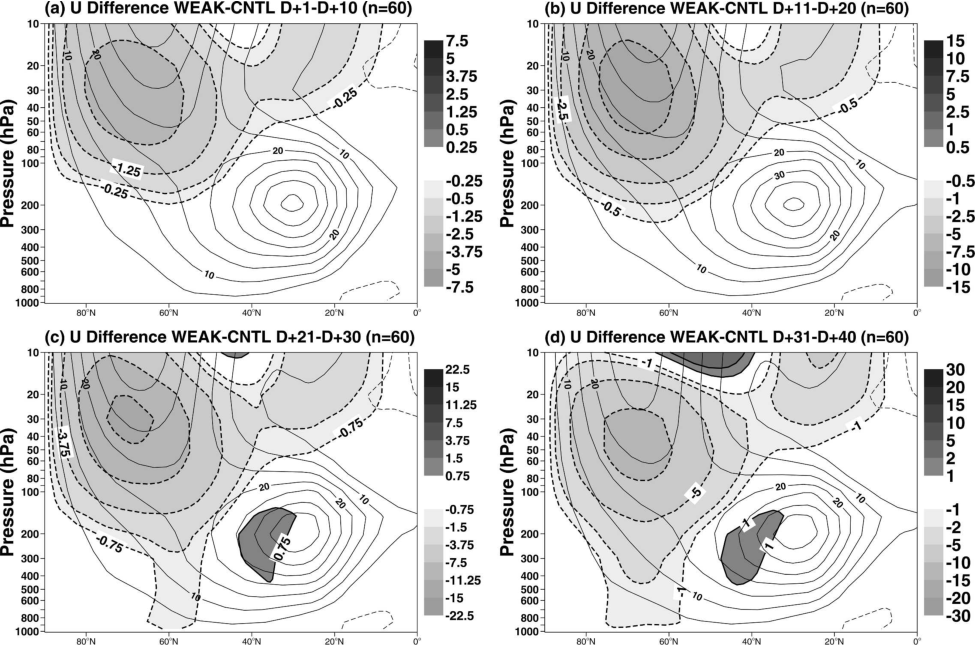
\includegraphics[width=\textwidth]{figures/chapter-intro/Jung_Barkmeijer.pdf}
 \caption[Numerical simulation results from \citet{Jung2006}]{Difference of
   average zonal-mean zonal winds (shading in $\mathrm{m~s^{-1}}$) between a
   weak polar vortex (WEAK) control experiment (CNTL) for 10-day averages
   following the start of the stratopheric forcing at time D: (a) D+1 to D+10,
   (b) D+11 to D+20, (c) D+21 to D+30, and (d) D+31 to D+40. Shown is the
   average over 60 different cases (40-day integrations). Notice that the
   contour interval for the differences changes linearly with the forecast
   range. Also shown are zonal-mean zonal winds from the control integration
   (contour interval is $\mathrm{5~m~s^{-1}}$). Figure from \citet{Jung2006}.}
 \label{fig:jung_barkmeijer}
\end{figure}

This tropospheric response to an imposed torque was shown to also operate on
long time scales by \citet{Scaife2005}. They found that when a long-term
acceleration of the stratospheric polar vortex was imposed from the
1960s--1990s, in line with observations, their model more faithfully reproduced
the long-term trend towards a more positive phase of the NAO over this time. It
is however, important to note that this does not necessarily imply that
stratospheric changes were driving the trend in reality.

In contrast to the studies above, which have calculated the tropospheric
response to an imposed stratospheric forcing, \citet{Simpson2011} removed the
stratospheric influence by nudging the polar stratosphere to a climatological
seasonal cycle. In doing so, they found that the effect of the stratosphere is
to lengthen SAM timescales\footnote{The SAM/NAM timescale is defined as the lag
  (in days) for its autocorrelation to fall by 1/$e$.} during the austral late
spring/early summer, and to lengthen NAM timescales during the boreal
winter-spring.

A criticism of studies with an imposed damping or torque is that they may not be
simulating a balanced, realistic, or physical state (for instance, the imposed
torque may not conserve angular momentum). As such, several studies have taken
place using free-running GCMs. \citet{Plumb2003} found using a simple
free-running stratosphere-only model that descending annular mode-like signals
of the kind shown in Figure \ref{fig:baldwin_dunkerton} can be simulated only by
changing the forcing at the lower boundary. They therefore conclude that
observations of this kind do not necessarily indicate a downwards influence from
the stratosphere. However, \citet{Gerber2008} undertook a similar study,
comparing relatively simple GCM simulations with varying representations of the
stratosphere. They altered the strength and variability of the stratospheric
polar vortex independently of the troposphere by varying the stratospheric lapse
rate, finding that simulations with a more variable polar vortex also had longer
timescales of the tropospheric NAM (a result similar to that of
\citet{Simpson2011}, although using a free-running model). This lengthened
timescale, in turn, was related to the long-lived tropospheric anomalies
following SSWs. Using the same model, \citet{Gerber2009} performed a series of
ensemble forecasts of model-simulated SSW events. They compared events in which
the initial tropospheric NAM was negative and positive, finding a negative NAM
to be much more likely following the SSW event in both cases. Hence, they
conclude that the stratosphere does indeed exert a significant downwards
influence on the troposphere in their model.

A further class of model investigation has been to compare models with a
well-resolved stratosphere with models with a coarser stratospheric resolution;
known as `high-top' and `low-top' models respectively \citep{Huebener2007,
  Sigmond2008, Cagnazzo2009, Sassi2010, Scaife2011, Charlton-Perez2013}
(discussed in greater detail in Section \ref{sec:models_introduction}). These
have all indicated a more realistic representation of tropospheric variability
and long-term trends is achieved with improved vertical
resolution. Additionally, in a case study of the cold European winter
2005--2006, \citet{Scaife2008} found increased blocking activity in a model with
greater stratospheric resolution. On the other hand, in a multi-model comparison
of blocking, \citet{Anstey2013} found a stronger relationship between blocking
frequency and upper-troposphere/lower-stratosphere vertical resolution than with
model lid height. Overall, large biases remain in models' representation of
blocking. A difficulty of these studies is that there are often several
differences between high- and low-top models besides their vertical resolution
(such as their parametrisation schemes), so it is difficult to pin down any
differences between the simulations to a stratospheric influence
alone. \citet{Hardiman2012a} attempted to address this issue by comparing model
simulations which differ only in their vertical resolution above 15~km. They
found the climatology and trends of surface temperature to be largely
insensitive to the increased vertical resolution, although stronger surface
anomalies following SSWs and a more realistic trend in the NAO were found in the
high-top model.

Several studies have investigated the influence of the stratosphere on the skill
of medium-range forecasts (also discussed in Section
\ref{sec:seas-introduction}). These have demonstrated improvements in the
medium-range predictive skill of high-top relative to low-top models
\citep{Marshall2010,Roff2011}, and enhanced predictability when forecasts are
initialised at the time of anomalously negative stratospheric NAM or SSWs
\citep{Kuroda2008,Mukougawa2009,Sigmond2013}. These studies therefore further
indicate a downwards influence of stratospheric variability on the troposphere. 



% Scaife and Knight cold 2006
% Simpson timescales
% blocking in models
% forecasts e.g. Charlton

\subsection{Mechanisms}
\label{sec:mechanisms}

The results described in the previous two sections provide strong evidence that
the stratosphere does indeed exert a significant influence on tropospheric
weather and climate. Even so, may uncertainties about the exact nature of the
influence remain; observational studies are always open to the criticism that
they do not demonstrate causality, and modelling studies that they contain large
model biases or are simulating an unrealistic scenario. A coherent picture of
stratosphere-troposphere coupling also requires a physical understanding of the
mechanism by which this takes place. Several such mechanisms have been proposed,
and are briefly described below:


\paragraph{Radiative effects.} It is well known that stratospheric (particularly
lower-stratospheric) temperature increases following SSWs lead to increasing
downwelling longwave radiation entering the troposphere.  \citet{Ramanathan1977}
argued that this warming could reduce the available potential energy accessible
to tropospheric eddy activity. Similarly, the stratospheric cooling associated
with ozone depletion leads to a reduction in downwelling longwave radiation
entering the troposphere \citep{Forster1997a}. \citet{Grise2009} used a
radiative transfer model to asses the impact of these radiation changes, finding
a significant impact on surface polar temperatures, although they did not assess
the circulation response. Indeed, relatively few studies have assessed the
impact of radiative processes in stratosphere-troposphere coupling in the light
of more recent observations. Despite this, it is unlikely that radiative effects
play a large role in the observed stratosphere-troposphere coupling since
relatively realistic coupling can be simulated in a model lacking interactive
ozone or a detailed radiation scheme.

\paragraph{Baroclinic instability.} The growth rate of baroclinic eddies is
related to the vertical shear in zonal wind throughout the troposphere
\citep{Eady1949}. Some studies have suggested that lower stratospheric zonal
wind anomalies which penetrate into the upper troposphere affect this vertical
wind shear, and so the growth of baroclinic eddies \citep{Wittman2007,
  Chen2008}. Hence, we may expect reduced tropospheric eddy activity at
mid-to-high latitudes following SSWs, due to weaker lower stratosphere/upper
troposphere zonal winds. \citet{Scaife2011} also used this relationship to
demonstrate that an increase in European winter storminess and equatorward shift
in the North Atlantic storm track projected under climate change are consistent
with a weakening and equatorward shift of the stratospheric polar vortex. It is
less clear whether the change in baroclinic eddy activity is sufficient to lead
to the annular mode signals of the kind shown in Figure
\ref{fig:baldwin_dunkerton}, although tropospheric eddies have been demonstrated
to be important in driving annular mode variability \citep{Limpasuvan1999}.

\paragraph{Downward control.} Under steady-state or time-mean conditions, the
`downward control' principle of \citet{Haynes1991} shows that the
streamfunction, $\psi$, of the TEM residual circulation is given by
\begin{equation}
  \psi(\phi,z) =
  \int_z^{\infty}\left(\frac{\rho_0a\overline{\mathcal{F}}\cos^2\phi}{\partial\overline{m}/\partial\phi}\right)_{\phi=\phi(z')}\mathrm{d}z'\, ,
\end{equation}
where $\overline{\mathcal{F}}$ is the total wave driving term from Equation
\ref{eq:zonal_momentum}, and
$\overline{m}=a\cos\phi(\overline{u}+a\Omega\cos\phi)$ is the angular momentum
per unit mass. Strictly, the integration is along a line of constant angular
momentum, but this is approximated as vertical (an approximation which breaks
down near the equator). Hence, it can be seen that under these conditions the
residual circulation at a given altitude depends only on the wave drag above
that altitude.

This relation therefore shows that circulation induced by stratospheric wave
drag extends to the Earth's surface, although it should be noted that the above
assumptions (particularly steady-state) do not strictly hold in the real
atmosphere. \citet{Thompson2006} suggested that this induced residual
circulation (or `balanced response') is sufficient to explain the observed
stratosphere-troposphere coupling. Others, however, have argued that the
observed annular mode-like tropospheric response cannot be generated in the
zonal-mean framework of downward control, necessitating feedbacks involving
tropospheric eddies \citep{Kushner2004, Song2004}.


\paragraph{Planetary wave reflection/refraction.} The critical surface formed in
the stratosphere during SSW events acts to reflect upward-propagating planetary
waves, as described in Section
\ref{sec:planetary-waves}. \citet{JudithPerlwitz2003} argued that these
reflected planetary waves re-enter the troposphere and affect the tropospheric
wave structures, leading to the observed tropospheric response. \citet{Shaw2010}
have further suggested that strong two-way coupling exists in the presence of
both a vertical reflecting surface and a strong meridional PV gradient, which
act to create a wave guide.

Other studies have suggested that it is the refraction of planetary waves at
lower levels, in the upper-troposphere/lower stratosphere (UTLS), that is most
important for communicating stratospheric anomalies to the surface
\citep{Limpasuvan2000,Hartmann2000}. Indeed, \citet{Chen1992} showed that
planetary wave propagation is very sensitive to small changes in this region
(also discussed by \citet{Haynes2005}).

\paragraph{Local adjustment to PV anomalies.} Under the QG approximation, PV
anomalies, $q'$, can be related to geopotential height anomalies, $Z'$, through
\begin{equation}
  q' = \mathcal{L}(Z')\, ,
\end{equation}
where $\mathcal{L}$ is a linear Laplacian-like operator \citep{Charney1962}. It
follows that the geopotential anomalies (and with QG approximations, other
dynamical fields) associated with a given PV anomaly can be derived by inverting
this operator. The geopotential height anomalies associated with a given PV
anomaly can be thought to be localised in that they decay with a typical
vertical and horizontal scales $H$ and $L$, which are the scale height and
horizontal scale of the QG flow respectively\footnote{It follows from this that
  PV-inversion is global in the sense that knowledge of the PV field everywhere
  is needed in order to fully determine the other dynamical fields.}. In the
case of lower-stratospheric PV anomalies, their influence may therefore extend
to the troposphere. \citet{Hartley1998} and \citet{Black2002} performed such
PV-inversions to calculate the tropospheric effect of stratospheric PV
anomalies. They found stratospheric PV anomalies to contribute significantly to
anomalies at the tropopause, which extend to the Earth's surface.

\begin{figure}
  \centering
  \noindent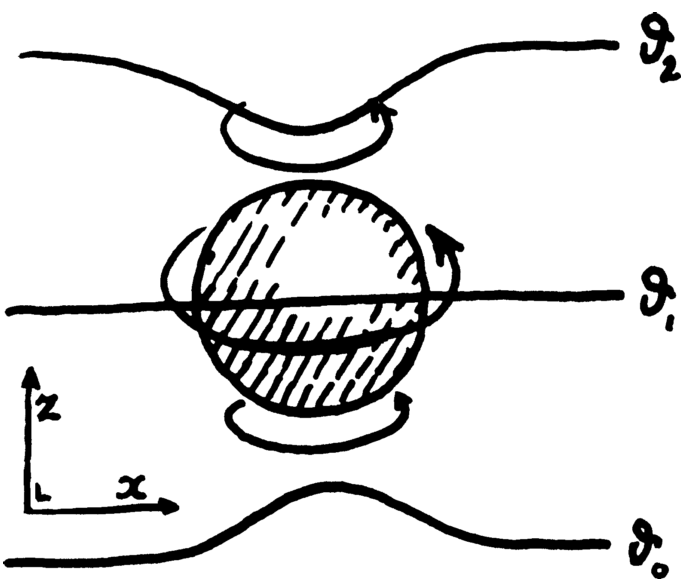
\includegraphics[width=0.4\textwidth]{figures/chapter-intro/ambaum_hoskins.png}
  \caption[Schematic from \citet{Ambaum2002}]{Schematic of the bending of
    isentropic surfaces (labelled $\theta_0$, $\theta_1$, and $\theta_2$) toward
    a positive potential vorticity anomaly. The arrows represent winds
    associated with the potential vorticity anomaly, becoming weaker away from
    the anomaly. Figure from \citet{Ambaum2002}.}
  \label{fig:ambaum_hoskins}
\end{figure}

It can be argued that PV-inversion does not constitute a `mechanism' since it is
not a time-dependent relationship and does not imply a direction of
causality. However, \citet{Ambaum2002} developed a physical mechanism analogous
to PV-inversion, as follows. Anomalies of PV act to bend isentropic surfaces
\citep{Hoskins1985}, as illustrated in Figure \ref{fig:ambaum_hoskins}. At high
latitudes, the tropopause lies approximately on a potential vorticity surface
\citep{Hoerling1991}, also the potential temperature of the tropopause will be
conserved for adiabatic changes (Section \ref{sec:planetary-waves}). Hence, the
tropopause will also bend in the presence of a stratospheric potential vorticity
anomaly; moving upwards for a positive anomaly, and downwards for a negative
anomaly. This deformation of the tropopause will then lead to hydrostatic and
geostrophic adjustment of the tropospheric column below, which can be thought of
in terms of the conservation of angular momentum, with a stretched tropospheric
column leading to an increase of vorticity and lower pressure. It is therefore
be expected that a strengthening of the stratospheric polar vortex would be
associated with negative sea-level pressure anomalies over the pole, and a
weakening with positive pressure anomalies, which is consistent with the
observed annular mode relationships (Section \ref{sec:observ-evid}).

Importantly, \citet{Ambaum2002} noted a stratosphere-leading time-lagged
relationship between the strength of the stratospheric polar vortex, the
tropopause height and the NAO, with the stratosphere acting to integrate the
NAO. This therefore represents a time-dependent and causal mechanism for
stratosphere-troposphere coupling.
\begin{center}
\line(1,0){250}
\end{center}

\bigskip The above list is not exhaustive but represents the most prominent
proposed mechanisms. It is clear that several of these mechanisms are not
mutually exclusive and so it is likely that more than one is at work in the real
atmosphere. Furthermore, a difficulty in distinguishing the relative importance
of the different mechanisms is that they are largely consistent with
observations, particularly in the tropospheric annular mode response to changes
in stratospheric polar vortex strength. It is therefore important to identify
situations in which mechanisms make different predictions and test these against
reality and numerical simulations.

One such situation is in the response to zonally asymmetric stratospheric
anomalies. For instance, the planetary wave reflection and downward control
mechanisms are largely sensitive only to zonal-mean quantities. Hence, it might
be expected that under these mechanisms the tropospheric response to two equal
zonal-mean stratospheric anomalies would be the same, even if the anomalies have
different zonal asymmetries. On the other hand, the tropospheric response via
adjustment to PV anomalies would be expected to be local to the stratospheric
anomalies.

It is the aim of Chapters \ref{cha:moments} and \ref{cha:models} to diagnose
zonally asymmetric stratospheric variability, specifically split and displaced
vortex events, in observations and model simulations. Part of the motivation for
this analysis is then to study the tropospheric response in order to test the
relative importance of the above mechanisms.

% Look at Song and Robinson 2004 for basis of mechanisms review
% Radiative Grise, Waugh
% SH coupling T&W


%\begin{figure}
% \centering
% \noindent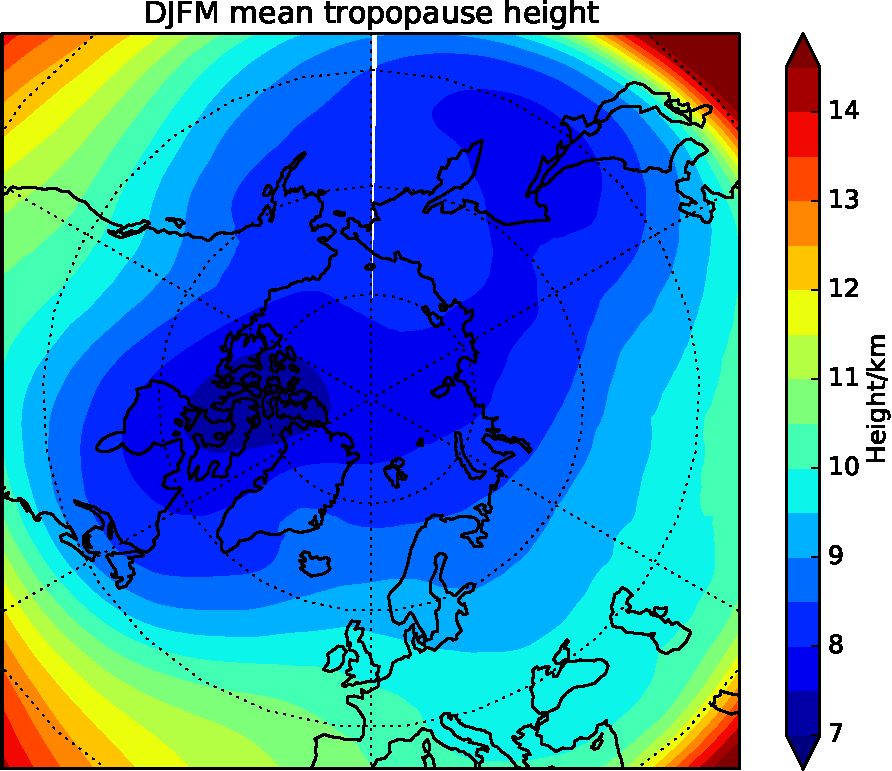
\includegraphics[width=0.5\textwidth]{figures/chapter-intro/mean_tropopause_height.pdf}
% \caption[]{ }
% \label{fig:cmip5_mslp_diff}
%\end{figure}



%%% Local Variables:
%%% mode: latex
%%% TeX-master: "thesis"
%%% End:







